\documentclass{standalone}

\usepackage{tikz}
\begin{document}
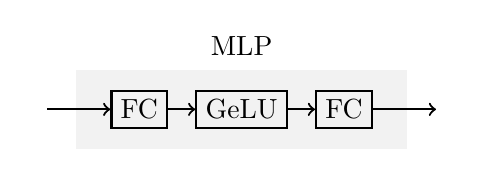
\begin{tikzpicture}[node distance=1.3cm, thick]
    \fill[gray!10] (0.5cm, 5mm) rectangle (4.7cm, -5mm);
    \node at (0, 0) (input){};
    \node[right of=input, shape=rectangle, draw] (fc1) {FC};
    \node[right of=fc1, shape=rectangle, draw] (gelu) {GeLU};
    \node[right of=gelu, shape=rectangle, draw] (fc2) {FC};
    \node[right of=fc2] (output){};
    \draw[->] (input) -- (fc1);
    \draw[->] (fc1) -- (gelu);
    \draw[->] (gelu) -- (fc2);
    \draw[->] (fc2) -- (output);
    \node at (2.6cm, 8mm) {MLP};
\end{tikzpicture}
\end{document}
